
\chapter{Enabling Technologies}
\label{chap:enabling_technologies}
\begin{chapterintro}
This chapter introduces which technologies have made possible this project. First of all there must be a place (repository) to store all the mash-ups, this is achieved by the OMELETTE mash-up register, explained in section \ref{sec:enableomr}. Second, the technology that has made possible feeding the repository in section \ref{sec:enableautomated}. Finally, the technologies that have been used to develop the web interfaces that enable browsing the mash-ups.
\end{chapterintro}

\cleardoublepage
\section{Overview}
In the current Web, developers enjoy the availability of plenty of services and widgets that can be reused to build new web applications. This ecosystem of reusable web components comprises elements such as data feeds of various domains, telco services or desktop and mobile widgets. Additionally, there is a growing set of tools for the creation of mash-ups such as MyCocktail~\cite{iglesias2011combining} or mashArt~\cite{daniel2009hosted} that facilitate developers in the combination of services into new applications. Also, Programmable Web, Yahoo Pipes or Opera widgets are examples of registries that reference services and widgets of many different kinds. Users can query them in order to search useful applications and services that they can reuse for mash-up composition.

However, developers face some difficulties when working on development of mash-ups. 

First, it is not easy for a developer to find the most appropriate services for a mash-up she is building, as although many of them are available but the information might be scattered across various repositories in the web in different formats on multiple levels of granularity.

Second, services are annotated using different description standards and semantics, thus requiring deep study of the documentation by the developer.

Third, due to this lack of consistent standardized descriptions, services need to be adapted in order to be used in a mash-up platform. 

This master thesis describes the creation of a searchable repository populated with services and widgets that will serve in wich a developer user will be able to find those components that he needs to create new mash-ups.

The main goal of this project is to create an interface that permits the developer fulfil his requisites finding the suitable services or widgets in the repository. To create this interface first there must be a repository and this repository must have widgets and services. The structure and the functionalities that this repository must have are described in section \ref{sec:enableomr} and we call it the OMELETTE mash-up Registry (OMR).

The repository is fed automatically using automated discovery techniques. These techniques are described in section \ref{sec:enableautomated} and exposed those existing websites on the Internet where the automatic algorithms fetch the data from.

\section{OMELETTE mash-up Registry}
\label{sec:enableomr}

The Omelette mash-up Registry (OMR) has a component model that aggregates necessary information for querying web components and searching the most appropriate ones. Additionally, this model reuses other underlying standards, such as WSMO, WSDL, WADL or W3C widgets, as low-level grounding standard description languages that allow components to be readily executable by referencing to them whenever available. These descriptions are built automatically, when possible, in a discovery phase that allows populating the registry with new reusable software artefacts from the Web.

Components stored in the OMR use the Linked mash-ups Ontology (LiMOn) RDF model~\cite{limon}.


\subsection{RDF model}
\label{subsec:rdfmodel}

The objective of the OMELETTE mash-up Registry is to provide an integrated centralized reference of web components to
facilitate querying and selection of relevant ones when building new mash-ups. To achieve this, an RDF model based format is employed to describe the components. It is defined in this section along with the interface that supports querying and selection of components from the registry.

\begin{figure}[ht!]
	\centering
	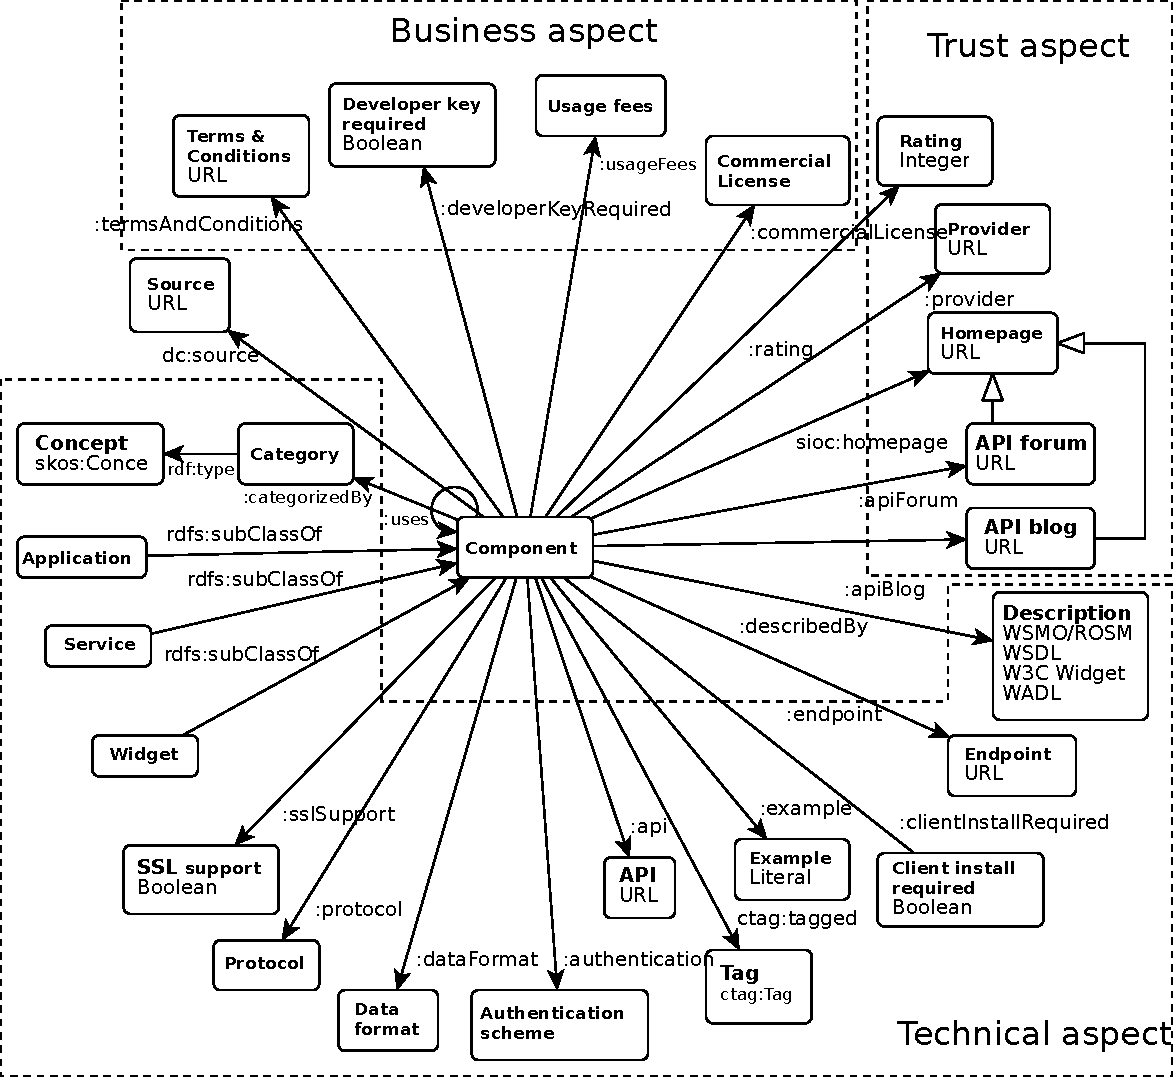
\includegraphics[width=400pt]{graphics/limon.pdf}
	\caption{Omelette mash-up Registry RDF model}
	\label{fig:omeletterdfmodel}
\end{figure}

The registry integrates heterogeneous components that can be potentially used in various web applications. More specifically, mash-up applications and services from the Web are the ones under consideration. mash-up is treated as a first-class object that is comprised of any web applications. Examples of mash-ups and services can be found in repositories such as Yahoo Pipes or Programmable Web.

In order to make these components available for developers, the registry stores relevant metadata that can be used by the developers for selecting components. Additionally, these metadata should be available in the web in order to make it possible to automate the population of the registry with real components. Usually, web component repositories contain metadata such as a component's name, textual description, tags or categorization. Other specific properties that depend on the nature of the component can also be found, such as inputs, endpoints, web service dependencies, or underlying formal descriptions like WSMO or WSDL.

With these considerations in mind, the OMELETTE team has defined the model presented in Figure \ref{fig:omeletterdfmodel}: LiMOn (Linked mash-up Ontology). It is a model that integrates the properties and fields that are provided by current component repositories in the web. Its name comes for its approach of bringing Linked Data to mash-up-Driven Development. It allows describing mash-ups and their components for integrating and sharing mash-up information such as categorization or dependencies.

This model covers aspects such as general categorization metadata, licensing or usage, and basic aspects of component execution. It reuses Simple Knowledge Organization System (SKOS\footnote{http://www.w3.org/2009/08/skos-reference/skos.html}), Friend of a Friend (FOAF\footnote{http://xmlns.com/foaf/spec/}), Dublin Core (DC\footnote{http://dublincore.org/}) and Common Tag (CTag\footnote{ttp://commontag.org/Home}) ontologies in order to follow the guiding principle of Semantic Web, which manifest reusability
as one of the main postulates.

The OMELETTE schema also makes use of work done in SOA4All~\cite{soa4all} FP7 project on RESTful services with ROSM/WSMO service descriptions. Every component might reference an additional description, such as WSDL, WSMO or W3C widget. As shown in the discovery section, ROSM will be used as the basis for describing REST services.

A registry with component descriptions according to the presented model can be queried using a SPARQL query as the one below:

\begin{lstlisting}[style=consola,caption={Example SPARQL}]
PREFIX om: <http://www.ict-omelette.eu/schema.rdf#>
PREFIX ctag: <http://commontag.org/ns#>
PREFIX rdfs: <http://www.w3.org/2000/01/rdf-schema#>

SELECT ?service
WHERE
{ ?service rdf:type om:Service;
	om:categorizedBy om:Telco;
	ctag:tagged [ rdfs:label "video" ];
	ctag:tagged [ rdfs:label "conference" ];
	om:developerKeyRequired "false". }
\end{lstlisting}

This query retrieves telco services with video conferencing functionality. The next SPARQL query asks the registry for services able to search a picture by keywords. It also retrieves the actual endpoint or URL that needs to be accessed to run the service:

\begin{lstlisting}[style=consola,caption={Example SPARQL keywords}]
PREFIX om: <http://www.ict-omelette.eu/schema.rdf#>
PREFIX ctag: <http://commontag.org/ns#>
PREFIX rosm: <http://www.wsmo.org/ns/rosm/0.1#>
PREFIX hrests: <http://www.wsmo.org/ns/hrests#>
PREFIX rdfs: <http://www.w3.org/2000/01/rdf-schema#>

SELECT ?service ?endpoint
WHERE
	{ ?service rdf:type om:Service;
	ctag:tagged
	[ rdfs:label "photos" ];
	om:describedBy [ rdf:type
	rosm:Service;
	rosm:requestURIParemeter [ ctag:tagged [ rdfs:label "keywords" ] ];
	hrests:hasAddress
	?endpoint ]. }
\end{lstlisting}


\section{Automated Discovery}
\label{sec:enableautomated}

Automated discovery is one of the tasks present in the scope of this project. Its objective is to enable OMELETTE users to access a wide amount of web components (i.e. both widgets and services) inside the OMR. Thanks to the automated discovery capabilities OMELETTE users will be able to use services and widgets as soon as they are published on external repositories.


\subsection{Introduction}

Three repositories were mined for services, widgets and mash-ups at this stage of the project,
namely Programmable Web\footnote{http://www.programmableweb.com/}, Opera Widgets\footnote{http://widgets.opera.com/} and Yahoo Pipes\footnote{http://pipes.yahoo.com/}.


\begin{description}
  \item[ProgrammableWeb] \hfill \\
  Programmable Web, shown in \ref{fig:programmableweb}, is the most popular registry of APIs and mash-ups on the Web, and allows developers to include their APIs or mash-ups for other developers. It currently contains more than 3,000 APIs and more than 5,000 mash-ups. Information about which APIs are used by mash-ups, licensing issues, or categorization information can be found in Programmable Web too.

\begin{figure}[ht!]
\centering
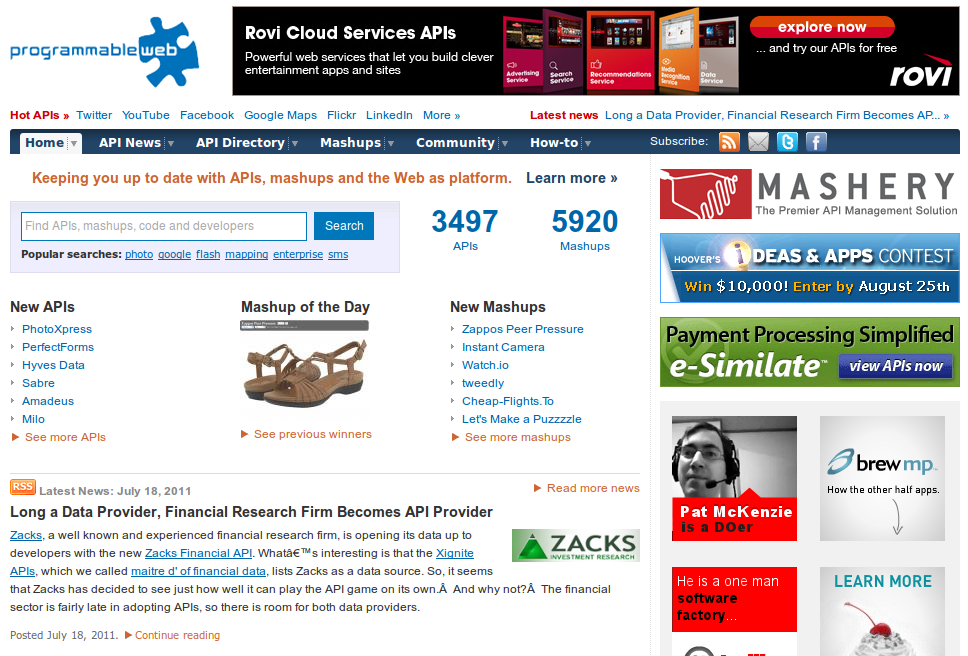
\includegraphics[width=400pt]{graphics/programmableweb.png}
\caption{ProgrammableWeb}
\label{fig:programmableweb}
\end{figure}
  
  \item[Yahoo Pipes] \hfill \\
  Yahoo Pipes, shown in \ref{fig:yahopipes}, is a mash-up environment developed by Yahoo, where developers can build data feeds that make use of other feeds by visually dragging and dropping operators and sources. The resulting so-called "pipes" can be run as any other feed, also accepting input parameters and providing a standardized RSS output. The pipes, or mash-ups, are categorized by tags, data format, sources, and also include short textual descriptions.

\begin{figure}[ht!]
\centering
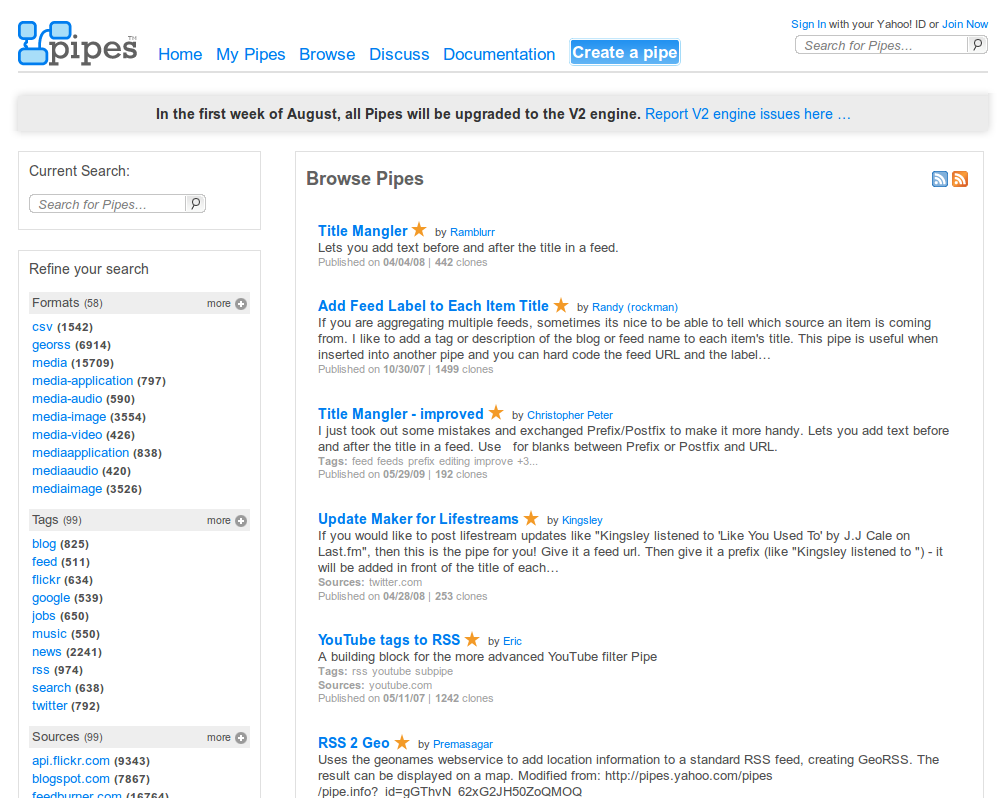
\includegraphics[width=400pt]{graphics/yahoopipes.png}
\caption{Yahoo Pipes}
\label{fig:yahopipes}
\end{figure}

  \item[Opera Widgets] \hfill \\
  Opera Widgets, shown in \ref{fig:operawidgets}, is a repository of mainly W3C widgets that are shared among the community of users of Opera Web Browser. These widgets can be used in OMELETTE because they follow W3C Widget standard. The repository provides a categorized collection of widgets, along with short textual descriptions of the widget's functionality.

\begin{figure}[ht!]
\centering
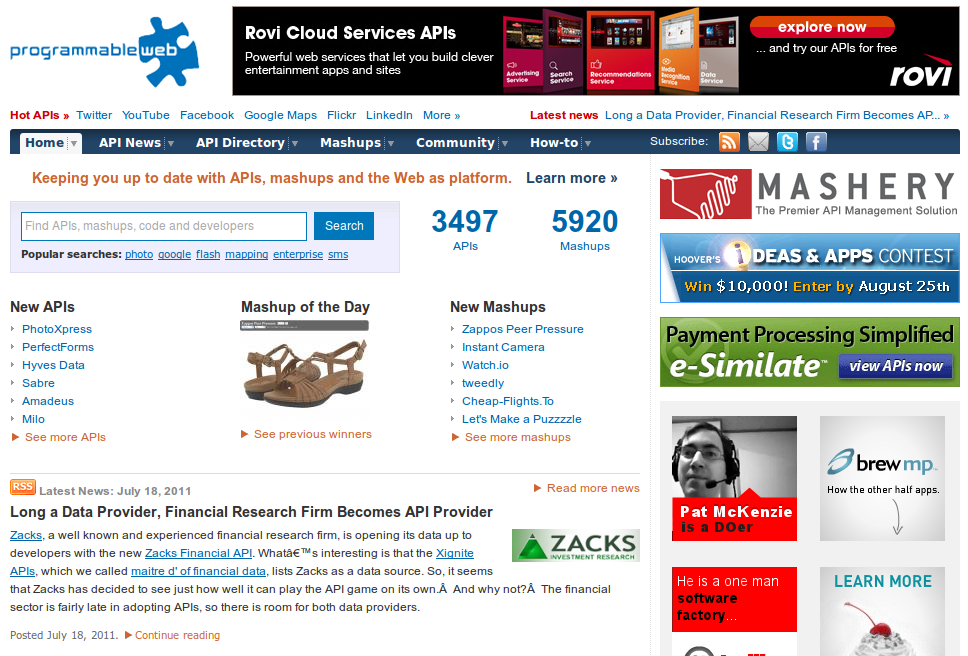
\includegraphics[width=400pt]{graphics/operawidgets.png}
\caption{Opera Widgets}
\label{fig:operawidgets}
\end{figure}
\FloatBarrier
\end{description}

\subsection{Discovery techniques}
\label{subsec:limonontology}

In order to mine the mentioned websites, a common approach was employed to extract the data. As part of the World Wide Web, the three repositories show a RESTful architecture, where a set of interlinked resources are published with resource specific descriptions. The format of the returned representations of the web resources is not standard, as they do not use any form of semantic annotations on top of the HTML data.

To map the HTML representations of the web resources available in these repositories to the RDF model defined for the OMELETTE mash-up Registry, the Scraping Ontology~\cite{fernandez2011semantic} ~\cite{scont11} has be used by the Open Source screen scraper called Scrappy ~\cite{scr11}, both developed in the context of OMELETTE.

Figure \ref{fig:mappingexample1} shows an example of mapping out of an unstructured HTML document into an OMELETTE RDF graph. In that example, a set of fragments in the HTML page are described along with the RDF data they represent. After processing that information on a particular sample HTML document, a scraper can produce the resulting RDF graph.

\begin{figure}[ht!]
\centering
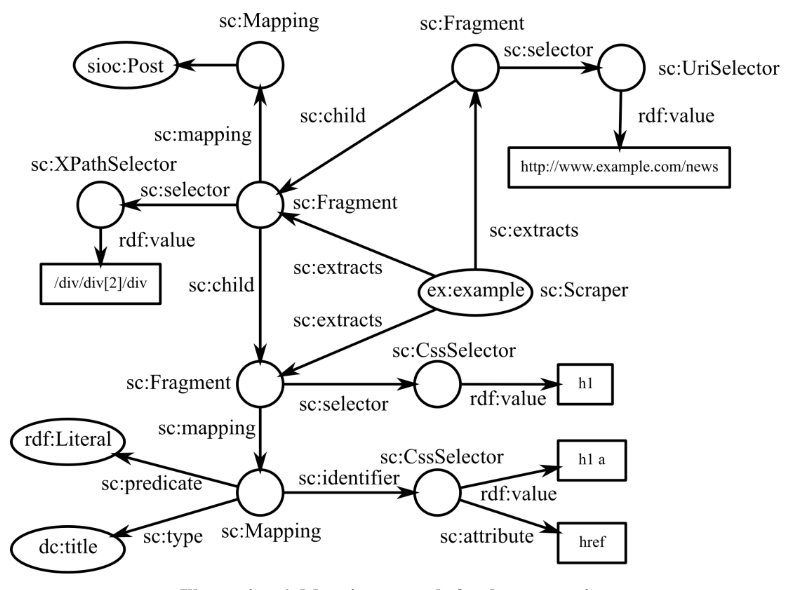
\includegraphics[width=350pt]{graphics/graph1.png}
\caption{Mapping example for data extraction}
\label{fig:mappingexample1}
\end{figure}

\begin{figure}[ht!]
\centering
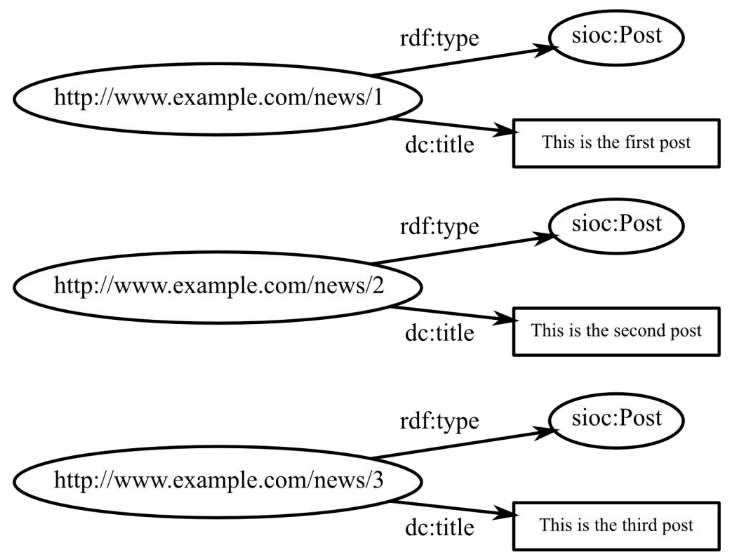
\includegraphics[width=350pt]{graphics/graph2.png}
\caption{Mapping example for data extraction}
\label{fig:mappingexample2}
\end{figure}


The methodology followed for the discovery assumes that first of all it is necessary to define a set of mappings for each of the repositories. These mappings state what data could be extracted, and how it could be done. Then prepared mappings are used by Scrappy to crawl the sites and build an RDF knowledge base that is dumped into the OMR.

In the case of Programmable Web, each web resource either represents a mash-up or an API. For each of them, the fields shown are mapped into an element of the ontology, covering the components' metadata such as categorization or tagging.

Similarly, for Opera Widgets each web resource represents a widget, so the information about the widget is mapped to the terms from the ontology. Also, its widget package (which uses WGT extension\footnote{http://www.w3.org/TR/2011/REC-widgets-20110927/}) is mapped as well as the widget's endpoint.

In Yahoo Pipes, more advanced scraping has been performed, thanks to an implicit service description that is available as an HTML form. For each pipe, a form for its execution is available in the mash-up's webpage, as shown in Figure \ref{fig:yahoopipesmash-up}.

\begin{figure}[ht!]
\centering
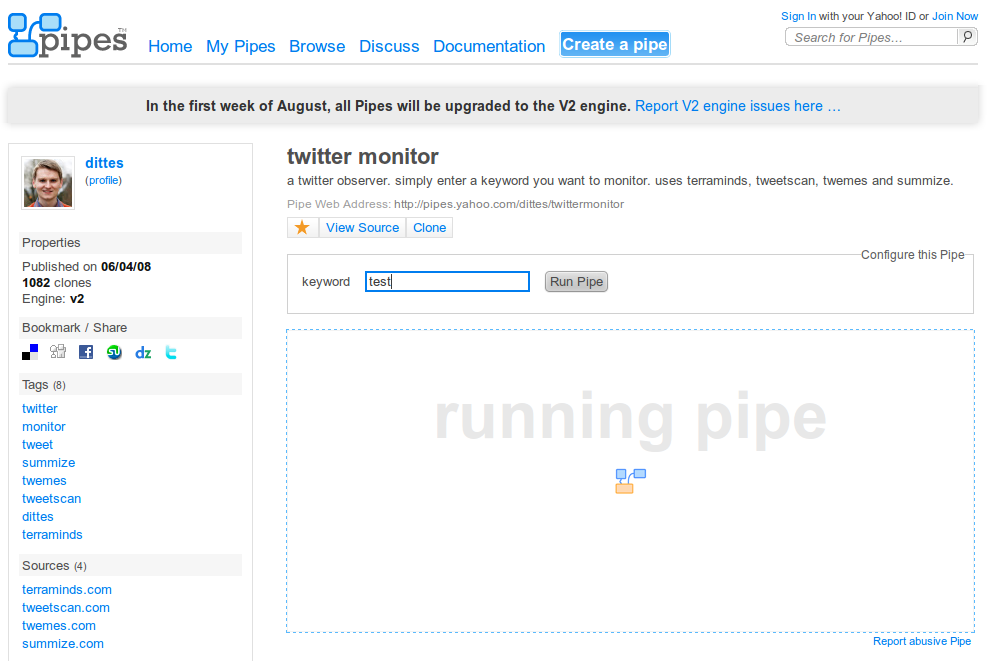
\includegraphics[width=350pt]{graphics/yahoopipesmashup.png}
\caption{Execution page of a Yahoo Pipe's mash-up}
\label{fig:yahoopipesmash-up}
\end{figure}

These HTML forms are mapped to a Resource-Oriented Service Model (ROSM) or a Web Service Modeling Ontology (WSMO) description in order to get detailed information of the
service's interface. 

\newpage
An example of ROSM description, extracted from the pipe shown in the Figure \ref{fig:mappingexample1}, which accepts a set of textual keywords on a URL, is shown next:


\begin{lstlisting}[style=listXML,caption={Example ROSM definition}]
<rosm:Service>
	<rosm:supportsOperation>
		<rosm:Operation>
			<hrests:hasAddress
			rdf:resource="http://pipes.yahoo.com/pipes/pipe.info?_id=c32fa09"/>
				<rosm:requestURIParameter>
					<rdf:Description>
						<ctag:tagged>
							<rdf:Description>
								<rdfs:label>text</rdfs:label>
							</rdf:Description>
						</ctag:tagged>
						<rdfs:label>keyword</rdfs:label>
				</rdf:Description>
			</rosm:requestURIParameter>
		</rosm:Operation>
	</rosm:supportsOperation>
</rosm:Service>

\end{lstlisting}

\section{Conclusions}

In this chapter we have introduces some of the technologies wich are part of the OMELETTE project and conform the base for this master thesis.

It is necessary to understand first what a repository is for and how the automated discovery is done. We have also introduced the websites scrapped and this helps to understand what kind of services and widgets populate the repository.





